% This is auto-generated file: do not edit!
% Exported from microMathematics Plus, version 2.19.0


Данный пример демонстрирует
построение трёхмерных графиков
для трёх различных функций двух
переменных.

Для начала, определим интервалы
изменения двух независимых
переменных x и y. Область
изменения переменной x зависит от
количества точек по оси абсцисс N,
а также от минимального и
максимального значений x1 и x2:
\begin{center}\begin{tabular}{ccc}
  $N := 300$ &
  $x1 := -2$ &
  $x2 := 2$ \cr
\end{tabular}\end{center}
\begin{center}\begin{tabular}{c}
  $x := \left[ x1,\, x1 +  \left| x2 - x1 \right|  / N \,..\, x2 \right]$
\end{tabular}\end{center}

Область изменения переменной y по
оси ординат определим аналогично:
\begin{center}\begin{tabular}{ccc}
  $M := 300$ &
  $y1 := -3$ &
  $y2 := 3$ \cr
\end{tabular}\end{center}
\begin{center}\begin{tabular}{c}
  $y := \left[ y1,\, y1 +  \left| y2 - y1 \right|  / M \,..\, y2 \right]$
\end{tabular}\end{center}

Первая функция является
произведением синуса и косинуса
степенных функций:
\begin{center}\begin{tabular}{c}
  $F(x,y) := sin \left( 3 \cdot {x}^{2}\right)  \cdot cos \left( {y}^{2}\right) $
\end{tabular}\end{center}

Для создания контурного графика
используйте кнопку ''Вставить'' на
верхней панели инструментов или
кнопку ''Вставить 3D график'' на
нижней панели:
\begin{center}\begin{tabular}{c} 
\includegraphics[width=0.45\textwidth]{graphics/three_d_plot_fig1.png} \end{tabular}\end{center}

В центральное поле внизу графика
вводится или имя функции с двумя
аргументами, или выражение,
которое явно зависит от двух
переменных интервального типа:
\begin{center}\begin{tabular}{c} 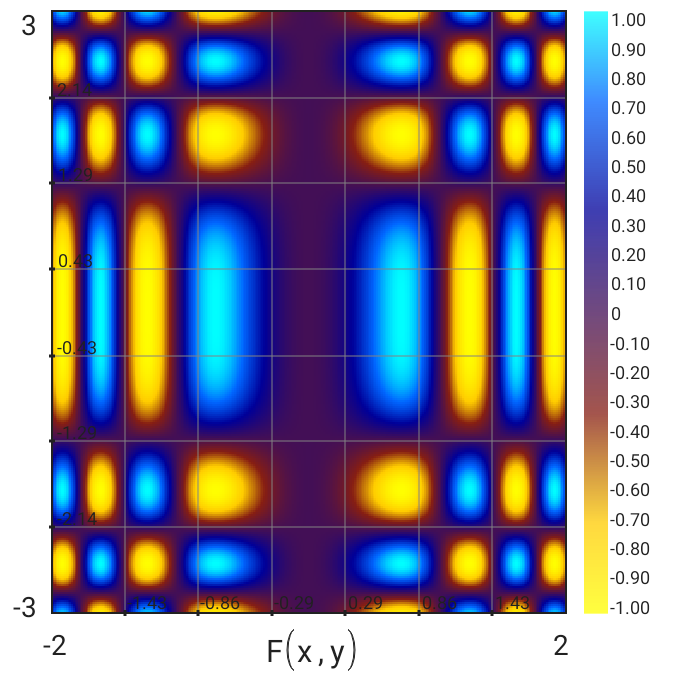
\includegraphics[width=0.45\textwidth]{graphics/three_d_plot_fig2.png} \end{tabular}\end{center}

Также же как и для графика функции
одной переменной, размер и стиль
трёхмерного графика изменяется в
окне настроек графика (см. пример
''График функции'' из навигатора
приложения). Это окно можно
вызвать кнопкой ''Настройки
объекта'', которая появляется при
долгом нажатием на центральную
область графика.

Дополнительно можно изменить
цветовую палитру и количество
маркеров по оси z. Это делается в
диалоговом окне ''Цветовая схема'',
которое вызывается долгим нажатием
на цветовую панель справа от
области графика.
\begin{center}\begin{tabular}{c}
  $R(x,y) := sin \left( 5 \cdot {x}^{2} \cdot \left( y - x \right)\right) $
\end{tabular}\end{center}
\begin{center}\begin{tabular}{c} 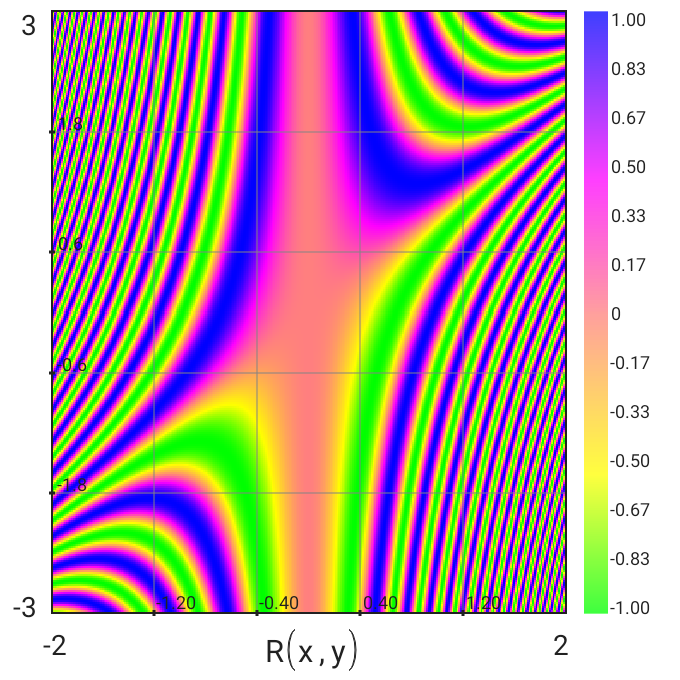
\includegraphics[width=0.45\textwidth]{graphics/three_d_plot_fig3.png} \end{tabular}\end{center}

Функцию двух переменных также можно
отобразить и в виде поверхности.
Этот режим отображения включается
в окне настроек графика. Как уже
говорилось, оно вызывается
нажатием на плавающую кнопку
''Настройки объекта'' после долгого
нажатия на поле графика. Для
примера, построим такую
поверхность, используя промежуточные
массивы для ускорения вычислений:
\begin{center}\begin{tabular}{cccc}
  $N := 100$ &
  $n := \left[ 0,\, 1 \,..\, N \right]$ &
  $x1 := -15$ &
  $x2 := 15$ \cr
\end{tabular}\end{center}
\begin{center}\begin{tabular}{cccc}
  $M := 100$ &
  $m := \left[ 0,\, 1 \,..\, M \right]$ &
  $y1 := -15$ &
  $y2 := 15$ \cr
\end{tabular}\end{center}
\begin{center}\begin{tabular}{c}
  $x[n] := {\left( x1 +  \left( x2 - x1\right)  \cdot n / N \right)}^{2}$
\end{tabular}\end{center}
\begin{center}\begin{tabular}{c}
  $y[m] := {\left( y1 +  \left( y2 - y1\right)  \cdot m / M \right)}^{2}$
\end{tabular}\end{center}
\begin{center}\begin{tabular}{c}
  $r[n,m] := 0.04 \cdot x_{n}  + 0.02 \cdot y_{m} $
\end{tabular}\end{center}
\begin{center}\begin{tabular}{c}
  $t[n,m] := \left( x_{n}  + 0.05 \cdot y_{m}  \right) \cdot exp \left( 1 - r_{n,\, m} \right) $
\end{tabular}\end{center}
\begin{center}\begin{tabular}{c}
  $F[n,m] := \frac{sin \left( x_{n}  + 0.1 \cdot y_{m} \right) }{0.15 + r_{n,\, m} } + \frac{t_{n,\, m} }{10}$
\end{tabular}\end{center}
\begin{center}\begin{tabular}{c} 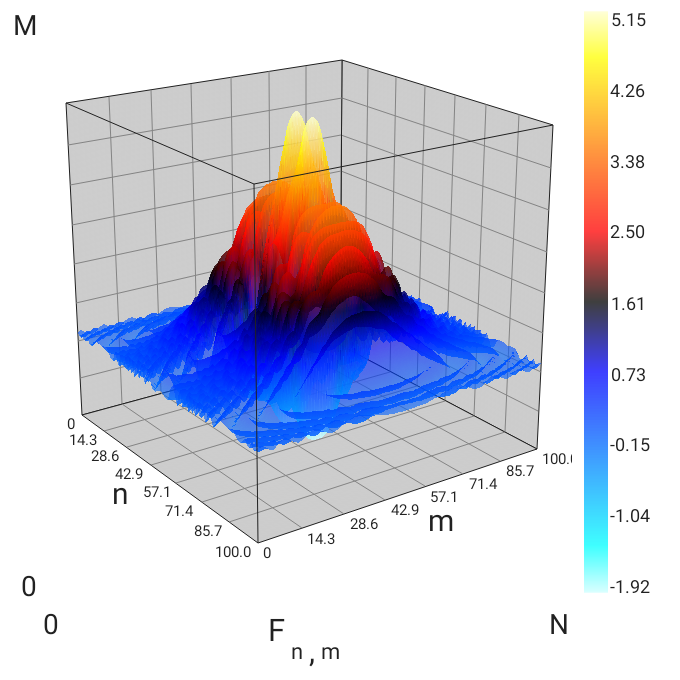
\includegraphics[width=0.45\textwidth]{graphics/three_d_plot_fig4.png} \end{tabular}\end{center}

Если функция отображается в виде
поверхности, то в окне ''Настройка
графика'' можно настроить для неё
дополнительные параметры: показ
линий сетки, режим закрашивания,
прозрачность, углы поворота и
наклона поверхности. Например,
посмотрим на предыдущую 
поверхность под другим углом:
\begin{center}\begin{tabular}{c} 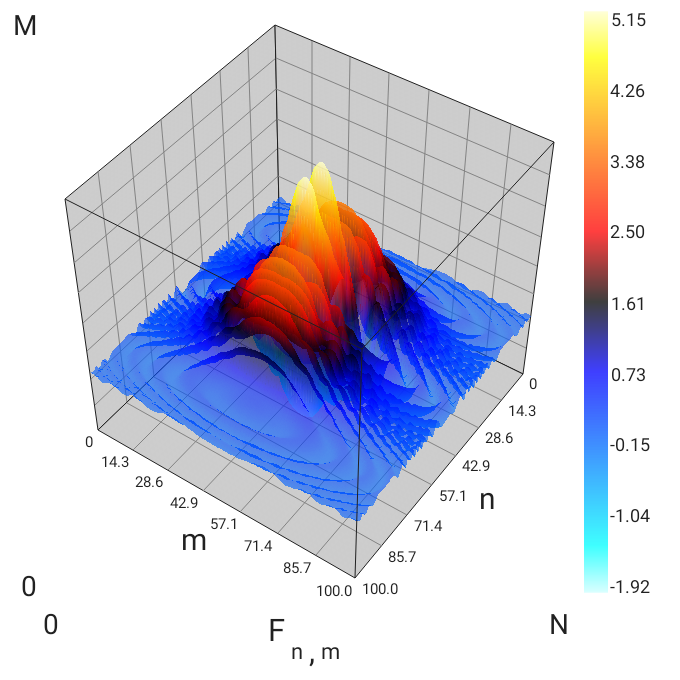
\includegraphics[width=0.45\textwidth]{graphics/three_d_plot_fig5.png} \end{tabular}\end{center}